\documentclass[11pt,a4paper]{report}
\usepackage{graphicx}
\graphicspath{{./images/}}
\usepackage[utf8]{inputenc}
\usepackage{amsmath}
%\usepackage{tabto}
\usepackage{amsfonts}
\usepackage{amssymb}
\usepackage{tikz-cd}
\usepackage{amsthm}
\usepackage{xcolor}
\usepackage[margin=1in]{geometry}
\linespread{1.25}
\usepackage[colorlinks=true,          % link colors, set to 'false' for print version
            linkcolor=blue,
            citecolor=red,
            urlcolor=blue]{hyperref}
            

%\setlength{\topmargin}{30mm}
%\addtolength{\topmargin}{-1in}
%\addtolength{\topmargin}{-\headsep}
%\addtolength{\topmargin}{-\headheight}
%\addtolength{\topmargin}{-\topskip}

%\setlength{\textheight}{270mm}
%\addtolength{\textheight}{\topskip}
%\addtolength{\textheight}{-\footskip}
%\addtolength{\textheight}{-30pt}

%\setlength{\oddsidemargin}{-1in}
%\addtolength{\oddsidemargin}{20mm}
%\setlength{\evensidemargin}{\oddsidemargin}

%\setlength{\textwidth}{170mm}

\newtheorem{defn}{Definition}[section]
 \newtheorem{thm}{Theorem}[section]
 \newtheorem{Lemma}{Lemma}[section]
 \newtheorem{Claim}{Claim}[section]
 \newtheorem{Prop}{Proposition}[section]
  \theoremstyle{definition}\newtheorem{Ex}{Example}[section]
 \newtheorem{Cor}{Corollary}[section]
 \newtheorem{claim}{Claim}[section]
 \newtheorem{conj}{Conjecture}  

\usepackage {amsfonts,amssymb}
%\usepackage{mathbbol}
\usepackage{latexsym}
\usepackage{mathrsfs}
\input xy
\xyoption{all}

\newcommand {\op}{\mathcal{O}\mathfrak{p}}
\newcommand {\Def}{\textrm{Def}}
\newcommand {\MC} {\textrm{MC}}
\newcommand {\Art}{\textrm{Art}_\CC}
\newcommand {\Kur}{\textrm{Kur}}
\newcommand {\LG} {^LG}
\newcommand{\fart}{\textrm{FArt}_\CC}
\newcommand{\fun}{\textrm{Fun}}
\newcommand{\sets}{\textrm{Sets}}
\newcommand{\tops}{\textrm{Top}}

\newcommand {\BB}{\mathbb{B}}
\newcommand {\CC}{\mathbb{C}}
\newcommand {\FF}{\mathbb{F}}
\newcommand {\KK}{\mathbb{K}}
\newcommand {\MM}{\mathbb{M}}
\newcommand{\NN}{\mathbb{N}}
\newcommand {\PP}{\mathbb{P}}
\newcommand{\QQ}{\mathbb{Q}}
\newcommand {\RR}{\mathbb{R}}
\newcommand {\SSS}{\mathbb{S}}
\newcommand {\VV}{\mathbb{V}}
\newcommand {\HH}{\mathbb{H}}
\newcommand {\WW}{\mathbb{W}}
\newcommand{\YY}{\mathbb{Y}}
\newcommand{\ZZ}{\mathbb{Z}}


\newcommand {\bal}{\boldsymbol{\alpha}}
\newcommand {\bbe}{\boldsymbol{\beta}}
\newcommand {\bga}{\boldsymbol{\gamma}}
\newcommand {\bmu}{\boldsymbol{\mu}}
\newcommand {\bom}{\boldsymbol{\omega}}
\newcommand {\bth}{\boldsymbol{\theta}}
\newcommand {\bph}{\boldsymbol{\phi}}
\newcommand {\bdh}{\boldsymbol{h}}
\newcommand {\bdk}{\boldsymbol{k}}
\newcommand {\bdE}{\boldsymbol{E}}
\newcommand {\bdU}{\boldsymbol{U}}
\newcommand {\bdP}{\boldsymbol{P}}
\newcommand {\ba}{{\bf a}}
\newcommand {\bb}{{\bf b}}
\newcommand {\bc}{{\bf c}}
\newcommand {\bd}{{\bf d}}
\newcommand {\bg}{{\bf g}}
\newcommand {\be}{{\bf e}}
\newcommand {\bdf}{{\bf f}}
\newcommand {\bp}{{\bf p}}
\newcommand {\bq}{{\bf q}}
\newcommand {\bv}{{\bf v}}
\newcommand {\bh}{{\bf h}}
\newcommand {\bk}{{\bf k}}
\newcommand {\br}{{\bf r}}
\newcommand {\bdu}{{\bf u}}
\newcommand {\bdv}{{\bf v}}
\newcommand {\bi}{{\bf i}}
\newcommand {\bj}{{\bf j}}
\newcommand {\bn}{{\bf n}}
\newcommand {\bs}{{\bf s}}
\newcommand {\bt}{{\bf t}}
\newcommand {\bu}{{\bf u}}
\newcommand {\bw}{{\bf w}}
\newcommand {\bx}{{\bf x}}
\newcommand{\by}{{\bf y}}
\newcommand {\bz}{{\bf z}}
\newcommand {\bB}{{\bf B}}
\newcommand{\bD}{{\bf D}}
\newcommand {\bE}{{\bf E}}
\newcommand {\bF}{{\bf F}}
\newcommand {\bG}{{\bf G}}
\newcommand {\bH}{{\bf H}}
\newcommand {\bK}{{\bf K}}
\newcommand {\bL}{{\bf L}}
\newcommand {\bM}{{\bf M}}
\newcommand {\bN}{{\bf N}}
\newcommand {\bO}{{\bf O}}
\newcommand {\bP}{{\bf P}}
\newcommand {\bQ}{{\bf Q}}
\newcommand {\bR}{{\bf R}}
\newcommand {\bT}{{\bf T}}
\newcommand {\bS}{{\bf S}}
\newcommand {\bU}{{\bf U}}
\newcommand {\bV}{{\bf V}}
\newcommand {\bW}{{\bf W}}
\newcommand {\bgamma}{\boldsymbol\gamma}
\newcommand {\bdelta}{\boldsymbol\delta}
\newcommand {\bDelta}{\boldsymbol\Delta}
%\newcommand{\qed}{{\ \bf qed}}

\newcommand {\rroot}{\mathbf{root}}
\newcommand {\coroot}{\mathbf{coroot}}
\newcommand {\weight}{\mathbf{weight}}
\newcommand {\coweight}{\mathbf{coweight}}
 \newcommand{\higgs}{\textrm{Higgs}}
\newcommand{\bun}{\textrm{Bun}}
\newcommand{\rk}{\textrm{rk}}
\newcommand{\ext}{\textrm{Ext}}
% \newcommand {\id}{\mathbb{1}}
% Use \id if using mathbbol instead of amssymb
\newcommand{\range}{\textrm{Range}}
\newcommand{\arccot}{\textrm{arccot}}

\newcommand{\thickslash}{\mathbin{\!\!\pmb{\fatslash}}}


\newcommand{\cA}{\mathcal{A}}
\newcommand{\cB}{\mathcal{B}}
\newcommand{\cC}{\mathcal{C}}
\newcommand{\cD}{\mathcal{D}}
\newcommand{\cE}{\mathcal{E}}
\newcommand{\cF}{\mathcal{F}}
\newcommand{\cG}{\mathcal{G}}
\newcommand{\cH}{\mathcal{H}}
\newcommand{\cI}{\mathcal{I}}
\newcommand{\cJ}{\mathcal{J}}
\newcommand{\cK}{\mathcal{K}}
\newcommand{\cL}{\mathcal{L}}
\newcommand {\cM}{\mathcal{M}}
\newcommand {\cN}{\mathcal{N}}
\newcommand {\cO}{\mathcal{O}}
\newcommand{\cP}{\mathcal{P}}
\newcommand{\cQ}{\mathcal{Q}}
\newcommand{\cR}{\mathcal{R}}
\newcommand{\cS}{\mathcal{S}}
\newcommand{\cT}{\mathcal{T}}
\newcommand{\cU}{\mathcal{U}}
\newcommand{\cV}{\mathcal{V}}
\newcommand{\cW}{\mathcal{W}}
\newcommand{\cX}{\mathcal{X}}
\newcommand{\cY}{\mathcal{Y}}
\newcommand{\cZ}{\mathcal{Z}}

\newcommand{\loc}{\mathcal{L}oc}
\newcommand{\Loc}{\textrm{Loc}}
\newcommand{\cih}{\mathpzc{h}}
\newcommand{\cx}{\mathpzc{x}}
\newcommand{\cy}{\mathpzc{y}}
\newcommand{\ce}{\mathpzc{e}}
\newcommand{\cf}{\mathpzc{f}}
\newcommand{\cl}{\mathpzc{l}}




 




\newcommand{\scA}{\mathscr{A}}
\newcommand{\scB}{\mathscr{B}}
\newcommand{\scC}{\mathscr{C}}
\newcommand{\scD}{\mathscr{D}}
\newcommand{\scE}{\mathscr{E}}
\newcommand{\scF}{\mathscr{F}}
\newcommand{\scG}{\mathscr{G}}
\newcommand{\scH}{\mathscr{H}}
\newcommand{\scI}{\mathscr{I}}
\newcommand{\scJ}{\mathscr{J}}
\newcommand{\scK}{\mathscr{K}}
\newcommand{\scL}{\mathscr{L}}
\newcommand{\scM}{\mathscr{M}}
\newcommand{\scP}{\mathscr{P}}
\newcommand{\scR}{\mathscr{R}}
\newcommand{\scO}{\mathscr{O}}
\newcommand{\scS}{\mathscr{S}}
\newcommand{\scT}{\mathscr{T}}
\newcommand{\scU}{\mathscr{U}}
\newcommand{\scV}{\mathscr{V}}
\newcommand{\scW}{\mathscr{W}}
\newcommand{\scX}{\mathscr{X}}
\newcommand{\scY}{\mathscr{Y}}
\newcommand{\scZ}{\scZ}

\newcommand{\uR}{\underline{\mathbb{R}}}
\newcommand {\uC}{\underline{\mathbb{C}}}


\newcommand{\fh}{\mathfrak{h}}
\newcommand{\fa}{\mathfrak{a}}
\newcommand{\fb}{\mathfrak{b}}
\newcommand{\fc}{\mathfrak{c}}
\newcommand{\fg}{\mathfrak{g}}
\newcommand{\fk}{\mathfrak{k}}
\newcommand{\fl}{\mathfrak{l}}
\newcommand{\fm}{\mathfrak{m}}
\newcommand{\fn}{\mathfrak{n}}
\newcommand{\fo}{\mathfrak{o}}
\newcommand{\fp}{\mathfrak{p}}
\newcommand{\fr}{\mathfrak{r}}
\newcommand{\fs}{\mathfrak{s}}
\newcommand{\fsu}{\mathfrak{su}}
\newcommand{\ft}{\mathfrak{t}}
\newcommand{\slt}{\mathfrak{sl}_2(\CC)}
\newcommand{\sln}{\mathfrak{sl}(n)}
\newcommand{\fsl}{\mathfrak{sl}}
\newcommand{\fu}{\mathfrak{u}}
\newcommand{\fv}{\mathfrak{v}}
\newcommand{\fx}{\mathfrak{x}}
\newcommand{\fy}{\mathfrak{y}}
\newcommand{\fz}{\mathfrak{z}}
\newcommand{\fA}{\mathfrak{A}}
\newcommand{\fB}{\mathfrak{B}}
\newcommand{\fD}{\mathfrak{D}}
\newcommand{\fM}{\mathfrak{M}}
\newcommand{\fR}{\mathfrak{R}}
\newcommand {\fU}{\mathfrak{U}}
\newcommand {\fV}{\mathfrak{V}}
\newcommand {\fW}{\mathfrak{W}}
\newcommand{\fX}{\mathfrak{X}}
\newcommand{\faff}{\mathfrak{aff}}

\newcommand{\Aff}{\textrm{Aff}}

\newcommand{\sym}{\textrm{Sym}}

\newcommand {\dbar}{\overline{\partial}}
\newcommand {\zbar}{\overline{z}}
\newcommand {\zvec}{\underline{z}}
\newcommand {\dzbar}{d\overline{z}}
\newcommand {\Nbar}{\overline{N}}
\newcommand {\Kbar}{\overline{K}}
\newcommand{\diff}{\textrm{Diff}}

%\newcommand {\hom}{\textrm{Hom}}

\newcommand{\mhom}{\textrm{Hom}}
\newcommand {\mend}{\textrm{End}}
\newcommand {\misom}{\textrm{Isom}}
\newcommand {\maut}{\textrm{Aut}}
\newcommand{\pr}{\textrm{pr}}

\newcommand {\sisom}{\underline{Isom}}
\newcommand {\saut}{\underline{Aut}}
\newcommand {\shom}{\textrm{\underline{Hom}}}
\newcommand {\send}{\underline{End} }

\newcommand{\dra}{M^{an}_{DR}(X,G)}
\newcommand{\dr}{M_{DR}(X,G)}

\newcommand {\ad}{\textrm{ad} }
\newcommand{\Ad}{\textrm{Ad}}

\newcommand{\lspan}{\textrm{span}}
\newcommand{\img}{\textrm{Im }}
\newcommand{\spec}{\textrm{Spec }}
\newcommand{\specan}{\textrm{Spec}^{an}}
\newcommand{\gspec}{\underline{\textrm{Spec }}}
\newcommand {\cok}{\textrm{coker}}
\newcommand{\tot}{\textrm{tot }}
\newcommand{\tildel}{\widetilde{\delta}}
\newcommand{\ctimes}{\otimes_\CC}
\newcommand{\sotimes}{\otimes_{\cO_X}}
\newcommand{\pic}{\textrm{Pic}}
\newcommand{\tr}{\textrm{tr }}

\newcommand  {\eps}{\varepsilon}
\newcommand {\kap}{\varkappa}
\newcommand {\io}{\iota}
\newcommand {\fii}{\varphi}

\newcommand{\Higgs}{{\bf Higgs}}
\newcommand{\Bun}{{\bf Bun}}
\newcommand{\gHiggs}{\op{\boldsymbol{\mathcal{H}iggs}}}
\newcommand{\Prym}{{\bf Prym}}
\newcommand{\Jac}{{\bf Jac}}
%\newcommand{\bh}{\boldsymbol{h}}
%\newcommand{\bH}{\boldsymbol{\mathcal{H}}}
\newcommand{\rts}{{\sf root}}
\newcommand{\wts}{{\sf weight}}
\newcommand{\crts}{{\sf coroot}}
\newcommand{\cwts}{{\sf coweight}}
\newcommand{\chr}{{\sf char}}
\newcommand{\cchr}{{\sf cochar}}

\newcommand{\Aut}{\textrm{Aut}}
\newcommand{\Der}{\textrm{Der}}
\newcommand{\spin}{\textrm{Spin}}
\newcommand{\spinc}{\textrm{Spin}^c}
%\newcommand{\U}{\boldsymbol{U(1)}}

\newcommand{\Mat}{\textrm{Mat}}

\newcommand{\hookr}{\hookrightarrow}

%%%%%%%%%%%%%%%%%%%%%%%%%%%%%%%%%%%%%%%%%%%%%%%%%%%%%%%%%%%%%%%%%%%%%%%%%
% Long exact sequence macro
%%%%%%%%%%%%%%%%%%%%%%%%%%%%%%%%%%%%%%%%%%%%%%%%%%%%%%%%%%%%%%%%%%%%%%%%%

\newcommand{\les}[9]{
\xymatrix{
 0 \ar[r] & {#1} \ar[r]  &  {#2} \ar[r]  &  {#3}
\ar@{->}`r/10pt[d] `[l] `^dl[dlll]  `^dr/10pt[dll]    [dll] \\
 &  {#4} \ar[r] & {#5} \ar[r] & {#6}
\ar@{->}`r/10pt[d] `[l] `^dl[dlll]  `^dr/10pt[dll]    [dll] \\
 & {#7} \ar[r]  & {#8} \ar[r] & {#9}
\ar@{->}`r/10pt[d] `[l] `^dl[dlll]  `^dr/10pt[dll]    [dll] \\
 & 0 \ar[r] & \cdots & }
}


%%%%%%%%%%%%%%%%%%%%%%%%%%%%%%%%%%%%%%%%%%%%%%%%%%%%%%%%%%%%%%%%%%%%%%%%%

\newcommand{\lestwo}[9]{
\xymatrix{     
 0 \ar[r] & {#1} \ar[r]  &  {#2} \ar[r]  &  {#3} 
\ar@{->}`r/10pt[d] `[l] `^dl[dlll]  `^dr/10pt[dll]    [dll] \\
 &  {#4} \ar[r] & {#5} \ar[r] & {#6} 
\ar@{->}`r/10pt[d] `[l] `^dl[dlll]  `^dr/10pt[dll]    [dll] \\
 & {#7} \ar[r]  & {#8} \ar[r] & {#9} }
}

%%%%%%%%%%%%%%%%%%%%%%%%%%%%%%%%%%%%%%%%%%%%%%%%%%%%%%%%%%%%%%%%%%%%%%%%%
% Long exact sequence macro
%%%%%%%%%%%%%%%%%%%%%%%%%%%%%%%%%%%%%%%%%%%%%%%%%%%%%%%%%%%%%%%%%%%%%%%%%

\newcommand{\lesthree}[5]{
\xymatrix{     
 0 \ar[r] & {#1} \ar[r]  &  {#2} \ar[r]  &  {#3} 
\ar@{->}`r/10pt[d] `[l] `^dl[dlll]  `^dr/10pt[dll]    [dll] \\
 &  {#4} \ar[r] & {#5} & }
}


%%%%%%%%%%%%%%%%%%%%%%%%%%%%%%%%%%%%%%%%%%%%%%%%%%%%%%%%%%%%%%%%%%%%%%%%%
% Long exact sequence macro
%%%%%%%%%%%%%%%%%%%%%%%%%%%%%%%%%%%%%%%%%%%%%%%%%%%%%%%%%%%%%%%%%%%%%%%%%

\newcommand{\lesfour}[8]{
\xymatrix{     
 0 \ar[r] & {#1} \ar[r]  &  {#2} \ar[r]  &  {#3} 
\ar@{->}`r/10pt[d] `[l] `^dl[dlll]  `^dr/10pt[dll]    [dll] \\
 &  {#4} \ar[r]^-{#8} & {#5} \ar[r] & {#6} 
\ar@{->}`r/10pt[d] `[l] `^dl[dlll]  `^dr/10pt[dll]    [dll] \\
 & {#7} \ar[r]  & \cdots  &  }
}

\newcommand{\equivclass}[1]{%
  #1/{\sim}%
}
\newcommand{\equivcls}[1]{%
  #1/\!{\sim}%
}

%


\include{biblio}
\author{Milos Vukadinovic}
\title{G(p,n) is a smooth manifold}
\begin{document}
Let us write $G(p,n) = \{ $p-dimensional (vector) subspaces of $\RR^{n \times p} \}$. A hyperplane $V \subseteq \RR^{n \times p}$ is specified by $n \times p$ matrix $A=[\vec{a}_1,\vec{a}_2, \dots, \vec{a_p}] \in Mat_{n\times p}$ where 
$\{\vec{a}_1, \vec{a}_2, \dots , \vec{a}_p \}$ is a basis for V. I.e., given $A \in Mat_{n\times p}$, $\rk A = p$, we get a p-hyperplane $V \subseteq \RR^{n \times p}$ by $V= $span $\{\vec{a}_1,\vec{a}_2, \dots, \vec{a}_p \} $. Conversely, given any p-dim subspace $V\subseteq \RR^{n \times p}$, there is a $n \times p$
matrix A with $\rk(A)=p$, from which $V$ is obtained in the above way. Two matrices, $A$ and $B$, determine the same subspace $V \iff \exists g \in GL(p) $, such that $B = A g$. $GL(p)$ stands for general linear group of degree $p$ over real field.
\newline
We thus have the following setup. Let the set of all \" 2-frames \" be
$$ F(p,n) = \{ A \; | \;  rkA=p \} \subseteq Mat_{n \times p}(\RR)  \simeq \RR^{n \times p} $$
and consider on it the equivalence relation
$$ B \sim A \text{ if } \exists \; g \in GL(p), \text{ s.t. } B=Ag $$
We have described a bijection of sets
$$ \equivclass{F(p,n)} \simeq  G(p,n). $$ 
We will show that $G(p,n)$ is a manifold equipped with a natural smooth structure. To achieve that we need to prove that:
\begin{itemize}
    \item $G(p,n)$ has a countable base
    \item $G(p,n)$ is Hausdorff
    \item $G(p,n)$ is locally euclidean
\end{itemize}
\begin{Prop}
    $F(p,n)$ is an open subset of $\RR^{p \times n}$
\end{Prop}
\begin{Lemma}\label{matrank}
    The rank of an $m \times n$ matrix is $r \iff$ some $r \times r$ minor does not vanish,
    and every $(r+1) \times (r+1)$ minor vanishes.
\end{Lemma}
Since we know that for $M \in F(p,n)^\complement$, $\rk M <p$ lemma \ref{matrank} tells us all $p \times p$ minors
of an arbitary element $ A \in F(p,n)^\complement$ vanish. Let's denote the determinant of each minor of $A$ with $S_i, \; i\in (1,2, \dots ,  {n \choose p})$ 
Then consider a continuous map
$ \psi: Mat_{n \times p} \to \RR^{ n \choose p}, \quad \psi(M) \to (S_1,S_2, \dots, S_{n \choose p})$.
We can express $F(p,n)^\complement = \psi ^{-1} ( \vec{0} )$ because all minors vanish (det=0).
A point $ \vec{0} \in \RR^{n \choose p}$ is a closed set, and because continuity preserves the closedness, $F(p,n)^\complement$ is closed in $Mat_{n \times p}$,
an since its complement is closed, $F(p,n)$ is an open subset of $Mat_{n \times p}(\RR)$
\begin{Prop}
    $\sim$ is an open equivalence relation on $F(p,n)$
\end{Prop}
In other words we need to show that the map $\pi: F(p,n) \to \equivclass{F(p,n)}$ is an open map.
Then $\pi$ is a quotient map and is equipped with $\equivclass{F(p,m)}$ is equipped with quotient topology.
\newline
\begin{Lemma} \label{quotientTop}
    A subset of a quotient space is open if and only if its
    preimage under the canonical projection map is open in the original topological space.
\end{Lemma}
Let $U$ be an open in $F(p,n)$. Then for every $g \in GL(p)$ the set $U g = \{ x g | x \in U \}$ is an open subset of $F(p,n)$.
Therefore $\pi^{-1}\pi(U) = \displaystyle \bigcup_{g \in G} \; U g$ is an open in $F(p,n)$ because the union of open sets is open.
And by \ref{quotientTop} $\pi(U) = [U]$ is open in $G(p,n)$. $\pi$ is a canonical quotient map, and $\equivclass{F(p,n)}$ is open in $\RR^{n \times p}$. 
\begin{Lemma}
    \label{baset}
    if $\beta = \{ \beta_\alpha \}_\alpha$ is a base for a topology $\mathcal{T}$ on a topological space $S$,
    and if $f: S \to X$ is an open map, then the collection $\{ f (\beta_\alpha) \}_\alpha$ is a base for the topology on $X$.
\end{Lemma}
\textbf{Proof:} Let $V$ be an open in $X$ and $y \in V$. Choose $x \in f^{-1}(y)$. 
Since $f^{-1} (V)$ is open there is a basis element $U \in \beta$ s.t. $x \in U \subset f^{-1}(V)$
which implies that $y \in f(U) \subset V$. Since $y$ is arbitary, and $f(U) \subset f(\beta)$ the collection $\{ f (\beta_\alpha) \}_\alpha$ is a base for the topology on $X$.
\newline
\newline
We have that $F(p,n)$ has a second countable base since it is a subspace of $\RR^{n \times p}$.
Thus by lemma \ref{baset}, we have that the base of $G(p,n)$ is second countable.
\begin{Prop}
The graph of the equivalence relation on $F(p,n)$ is a closed subset of $F(p,n) \times F(p,n)$. i.e. $ R = \{ (A,B) \in F(p,n) \times F(p,n) \; | \; A = Bg \}$ is closed.
\end{Prop}
We can consider $R$ as a set of matrices $[A B] = [\vec{a}_1, \vec{a}_2, \dots, \vec{a}_p, \vec{b}_1, \vec{b}_2, \dots , \vec{b}_p]$ of rank $p$.
Lemma \ref{matrank} tells us that every $(p+1) \times (p+1) $ minor of an element in $R$ must vanish. Consider the map that assigns to $(A,B)$ the values of all $ (p+1) \times (p+1) $ minors
$$ \psi:  F(p,n) \times F(p,n) \to \RR^{ {n \choose 3} (p+2) }$$
Since $\phi$ is continuous ( as all of its components are polynomials )  and $R = \psi^{-1} (0) $ , then R is closed.
\begin{Ex}
    For example take $G(2,4)$, then $\phi: Mat_{4 \times 2} \to \RR^{16}$ 
\end{Ex}
\begin{center}
      \centering
      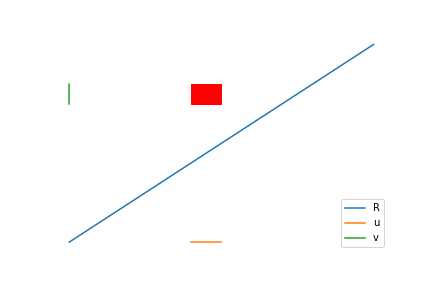
\includegraphics[width=0.90\textwidth]{graph_int.png}
\end{center}

\begin{Prop}
$G(p,n)$ is Hausdorff.
\end{Prop}

That is because $R$ is closed in $F(p,n) \times F(p,n)$, $(F(p,n) \times F(p,n)) \setminus R = R^{\complement}$ is open.
$\implies \forall (x,y) \in R^{\complement} $ there is a basic open set $u \times v$ containing $(x,y)$ s.t. $ (u \times v) \cap R = \emptyset 
\implies \forall x, y \text{ s.t. } (x,y) \not\in R, \exists$ u around x and v around y s.t. $u \cap v = \emptyset$
Thus for any two points $[x] \neq [y] \in \equivclass{F(p,n)}$ there exist disjoint neighborhood of $x$ and $y$ and $ \equivclass{F(2,4)}$ which is exactly the definition of Hausdorff property.
\newline
\begin{Prop}
   $G(p,n)$ is locally euclidean. 
\end{Prop}
Now that we have Hausdorff property and secound countable basis, we need to prove that every point lying on a manifold has a neighbourhood that is homeomorphic to an open in $\RR^n$.
Then we can claim that $G(p,n)$ is a manifold.
\newline
First we define charts. Take $A \in Mat_{n \times p} $ denote by $A_{k}$, ($ k \in \text{ all possible picks of p from the set } [1, \dots , n] $) the $p \times p$ minor, formed by the $k_1$th $\dots k_p$th rows of $A$.
The set
$$ U_{k} = \{ A \; | \; \det(A_{k}) \neq 0 \} \subset F(p,n)$$ is open, because its complement is closed. 
We also have that $\forall g \in GL(p)$ if $A \in U_{k}$ then $ Ag \in U_{k}$. 
Indeed, because $\det(Ag) = \det(A) \det(g)$, $\det( (Ag)_{i,j}) \neq 0$ which means $Ag$  will belong to a set $U_{k}$ 
Next, define
$$V_{k} = \equivclass{U_{k}} = \pi (U_{k}) \subset G(p,k)$$
The set $V_{k}$ is open since the equivalence relation is open. i.e. $\pi$ is an open map.
\newline
$U_k$ has a canonical representative $A \sim \widehat{A A_{k}^{-1}}$. $\widehat{\cdot}$ discards all the rows whose index is in $k$.
Similarly $V_k$ has a canonical representative: $[A] \sim [\widehat{A A_{k}^{-1}}] $

\begin{Ex}
Following the previous example consider $ [A] \in G(2,4)$.
If a minor $A_{2,4}$ is invertible we have that
$
[A] \sim [\widehat{A A_{2,4}^{-1}}] = 
\widehat{\begin{bmatrix}
* & * \\
1 & 0 \\
* & * \\
0 & 1
\end{bmatrix}} = \begin{bmatrix}  * & * \\ * & * \end{bmatrix}
$.
Since charts $ \bigcup U_k$ cover $F(p,n)$, charts $V_k$ cover $G(p,n)$ (because $\pi$ is open).
\end{Ex}
Now we define homeomorphisms between charts $V_k$ and opens in $R^{p \times (n-p)}$ as follows:
$$ \phi_{k}: V_{k} \subset G(p,n) \to Mat_{ (n-p) \times p} (\RR) \simeq \RR^{ (n-p) \times p) }, \quad \phi_{k}([A]) = \widehat{A A_{k}^{-1}} $$
We can show that $\phi$ is well defined. 
\newline
Let $A, A^\prime \in [A]$ we will show that $\phi$ is well defined. Equivalently $\phi_{k}(A) = \phi_{k}(A^\prime])$
Since $A$ and $A^\prime$ are in the same class, we have that $A^\prime = A g, \quad g \in GL(p) $, $\phi_{k}(A) = A A_{k}^{-1}$.
$$ \phi_{k}(A^\prime) = \phi_{k}(A g) = Ag ((Ag)_{k})^{-1} = Ag( A_{k} g )^{-1} = A g g^{-1} A_{k}^{-1} = A I A_{k}^{-1} = A A_{k}^{-1} = \phi_{k}(A) $$

$\phi$ is continuous because matrix multiplication is continous. Next, we can see that $\phi$ is surjective and $\phi^{-1}$ is continuous by explicitly defining inverse.

$$\phi_{k}^{-1}(\begin{pmatrix} \text{--- } \alpha_{1} \text{ ---}  \\ \vdots \\ \text{--- }  \alpha_{n-p} \text{ ---} \end{pmatrix}) =
\begin{pmatrix} 1_1 \\ \vdots  \\ 1_p \\ \alpha_1 \\ \vdots \\  \alpha_{n-p}  \end{pmatrix} $$
Finally, to show that $\phi$ is a homeomorphism,
we have left to shot that $\phi$ is injective. 
\newline
Assume that there $\phi_{k}$ is not injective then there are $A \in [A]$ and $B \in [B]$ such that there is \textbf{no} $g \in GL(p)$
for which $A g =  B$. i.e. $A A_{k}^{-1} = B B_{k}^{-1} \; \iff  \; 
 A A_{k}^{-1} B_{k} = B$ but $A_{k}^{-1} B_{k} \in GL(p)$ thus we reach contradiction.
Therefore $\phi_{k}$ is homeomorphism
\newline 
\begin{Ex} \label{ex1}
    Let $A = \begin{bmatrix}
        2 & 6 \\
        1 & 3 \\
        2 & 1 \\
        4 & 3 \\
    \end{bmatrix}, \quad [ A ] \in V_{3,4}$
    $$ A A_{3,4}^{-1} =  \begin{pmatrix} 2 & 6 \\ 1 & 3 \\ 2 & 1 \\ 4 & 3 \\ \end{pmatrix} \begin{pmatrix} \frac{3}{2} & -\frac{1}{2} \\ -2 & 1 \\ \end{pmatrix}
    = \begin{pmatrix} -9 & 5 \\ -\frac{9}{2} & \frac{5}{2} \\ 1 & 0 \\ 0 & 1 \end{pmatrix}
    $$
    the above multiplication is continuous by \ref{quotientTop} and we can exlcude rows $3$ and $4$ so that we get result in $R^4$.
    Then the restriction to $R^4$ is also continuous.
    $$ \phi_{3,4}([A]) = \begin{pmatrix} -9 & 5 \\ -\frac{9}{2} & \frac{5}{2} \end{pmatrix} $$
\end{Ex}
Next the inverse map  $\phi_{3,4}(\beta)^{-1} \; \beta \in Mat_{2 \times 2} = \phi_{3,4}(A_{1,2} A_{3,4}^{-1} g) = [A] $ for some matrix $A$, such that $A_{1,2} = \beta$.
But if we pick $g = A_{3,4}$ then 
$ \phi_{3,4}(\beta) =
\begin{bmatrix}
    \beta_{1,1} & \beta_{1,2} \\ 
    \beta_{2,1} & \beta_{2,2} \\
    1 & 0 \\ 
    0 & 1 \\
\end{bmatrix}
$
More generally
$$\phi_{i,j}^{-1} : \RR^4 \to v_{i,j} \subset G(2,4) \quad \phi_{i,j}^{-1}(\beta) \to 
\begin{bmatrix}
    \beta \\
    I_{2 \times 2}
\end{bmatrix} = [\alpha]
$$
Such that $\alpha [i:] = \beta[1:]$, $\alpha[j:] = \beta[2:]$ , $\alpha[ (I \setminus \{i,j\})[1] ] = I[1:]$ and
$\alpha[ (I \setminus \{i,j \})[2] ] = I[2:]$
\newline
\begin{Ex}
   $ \phi_{3,4}^{-1} (\alpha) = [A] $ as defined in \ref{ex1}
   $$ \phi_{3,4}^{-1}  \begin{pmatrix} -9 & 5 \\ -\frac{9}{2} & \frac{5}{2} \end{pmatrix} = \begin{bmatrix} -9 & 5 \\ -\frac{9}{2} & \frac{5}{2} \\ 1 & 0 \\ 0 & 1 \end{bmatrix} $$ 
   We can confirm that $ \alpha = \begin{bmatrix} -9 & 5 \\ -\frac{9}{2} & \frac{5}{2} \\ 1 & 0 \\ 0 & 1 \end{bmatrix}$ and $A = \begin{bmatrix}
        2 & 6 \\
        1 & 3 \\
        2 & 1 \\
        4 & 3 \\
    \end{bmatrix}$
    span the same subspace.
    Because if we take $g = \begin{pmatrix} 2 & 1 \\ 4 & 3 \\ \end{pmatrix}$
    then $\alpha g = A$
\end{Ex}
Since $\bigcup U_{i,j}$ covers $F(2,4)$, $\cup v_{i,j}$ covers $G(2,4)$
Finally, we check transition maps.
$$ \phi_{1,2}([A])^{-1} = A_{3,4} A_{1,2}^{-1}, \quad \phi_{1,2}^{-1}(u) =
\begin{pmatrix}
1 & 0 \\
0 & 1 \\
v_{1,1} & v_{1,2} \\
v_{2,1} & v_{2,2}
\end{pmatrix}
$$

$$ \phi_{2,4}([A]) = A_{1,3} A_{2,4}^{-1}, \quad \phi_{2,4}^{-1}(v) = 
\begin{pmatrix}
v_{1,1} & v_{1,2} \\
1 & 0 \\
v_{2,1} & v_{2,2} \\
0 & 1
\end{pmatrix}
$$
$$ \phi_{2,4} \circ \phi_{1,2}^{-1}(v) = 
\begin{pmatrix}
v_{1,1} & v_{1,2} \\
v_{2,1} & v_{2,2}
\end{pmatrix} =
\begin{pmatrix}
    1 & 0 \\
    v_{1,1} & v_{1,2}
\end{pmatrix}
\begin{pmatrix}
    0 & 1 \\
    v_{2,1} & v_{2,2}
\end{pmatrix} ^{-1}
= 
\begin{pmatrix}
    1 & 0 \\
    v_{1,1} & v_{1,2}
\end{pmatrix}
\begin{pmatrix}
    v_{2,2} & -1 \\
    -v_{2,1} & 0
\end{pmatrix} \frac{1}{-v_{2,1}} = 
$$
$$ -\frac{1}{v_{2,1}} \begin{pmatrix} v_{2,2} & -1 \\ v_{1,1} v_{2,2} - v_{1,2} v_{2,1} & -v_{4} \end{pmatrix}
$$
\newline
Now let's check the transition map $ \phi_{3,4} \circ \phi_{2,3}^{-1} $ 
$$ \phi_{3,4} \circ \phi_{2,3}^{-1} (v) =
\begin{pmatrix} v_{1,1} &  v_{1,2} \\ 1 & 0 \end{pmatrix} 
\begin{pmatrix} 0 & 1 \\ v_{2,1} & v_{2,2} \end{pmatrix} = 
-\frac{1}{v_{2,1}} \begin{pmatrix} v_{1,1} v_{2,2} + v_{1,2} v_{2,1} & -v_{1,1} \\ v_{2,2} & -1 \end{pmatrix}
$$ 
Hence $G(2,4)$ can be equipped with the structure of a 4 dimensional smooth manifold.
\newline
However, we can also consider $G(2,4)$ as a quotient of Stiefel Manifold.
We will define a Stiefel manifold as a set of orthonormal $k$ frames. 
$$V(n,k) \subseteq F(n,k); \quad V(n,k) = \{ A \; | \; rkA=2, \; A^T A = I \}$$
\begin{center}
\begin{tikzcd}
V(2,4) \arrow[r, hook] \arrow[dr, dashrightarrow, "p"]
& F(2,4) \arrow[d, "\pi"]\\
& G(2,4)
\end{tikzcd}
\end{center}
Map $p$ is surjective because every subspace has an orthonormal basis.
I.e. starting with any basis we can construct an orthonormal one via Gram-Schmidt algorithm.
Now, if we redefine the map $p$ such that $p: { F(2,4) / _{O(2)}} \to G(2,4)$, where $O(2)$
is the orthogonal group of $2-frames$, we will have a bijection. 
Therefore there are two ways we can consider $G(2,4)$
$$ G(2,4) = F(2,4) / _{Gl_2(\RR)} \quad G(2,4) = V(2,4) / _{O(2) }$$
\chapter{Tangent Spaces}
Let's define tangent spaces on $G(2,4)$. 
First consider the equivalence relation defined as:
$$ (p, (U,\phi), v) \sim (p, (V, \psi), w) \text{ if } w = J( \psi \circ \phi^{-1})_{\phi(p)} v $$
Consider tanget space on $G(2,4)$ at $X$, it's given by 
$$ T_p X = \equivclass{\{ (p,(U,\phi),v) \;|\; (U,\phi) \text{ is a chart around } p, v \in \RR^n \}} $$
Hence a tangent vector to $G(2,4)$ at $p \in G(2,4)$ is an equivalece class $ [ (p; (U; \phi); v)] $  
Whenever we have fixed the chart $(U; \phi)$, the class is represented just by a vector $v \in \RR^n$.
To represent the same equivalence class in another chart, we multiply $v \in \RR^n$ by the respective Jacobi matrix.
\newline
Jacobi matrix of transition map $\phi_{3,4} \circ \phi_{2,3}^{-1}$ is given by:
$$ J(\phi_{3,4} \circ \phi_{2,3}^{-1}) = 
\begin{pmatrix} 
    -v_{2,2} & 1 & 0 & -v_{1,1} \\
    \frac{1}{v_{2,1}} & 0 & -\frac{v_{1,1}}{v_{2,1}^2} & 0 \\
    0 & 0 & \frac{v_{2,2}}{v_{2,1}^2} & -\frac{1}{v_{2,1}} \\
    0 & 0 & -\frac{1}{v_{2,1}^2} & 0 
\end{pmatrix} $$
\begin{Ex}\label{tangentSpaces}
Consider the matrix a from the example \ref{ex1}. 
We have that $\phi_{3,4}([A]) = \begin{pmatrix} -9 & 5 \\ -\frac{9}{2} & \frac{5}{2} \end{pmatrix}$ and   
$\phi_{2,3} = \begin{pmatrix} 2 & 0 \\ 0.4 & 1.8 \end{pmatrix}$
$$ J(\phi_{3,4} \circ \phi_{2,3}^{-1}) =
\begin{pmatrix} 
    -1.8 & 1 & 0 & 0 \\
    2.5 & 0 & -12.5 & 0 \\
    0 & 0 & 11.25 & -2.5 \\
    0 & 0 & -6.25 & 0
\end{pmatrix} $$
Then 
$$ (p, (U,\phi_{2,3}), v) \sim (p, (V, \phi_{3,4}), w) \text{ if } w = J( \phi_{3,4} \circ \phi_{2,3}^{-1})_{\phi_{2,3}(p)} v $$
\end{Ex}
\textbf{How to project on such tangent spaces ?}
\newline
\chapter{$Gr(2,4)$ is compact}
We'll endow $R^{n \times k} $ with the norm induced by the
Frobenius inner product:
$$ || A || = \sqrt{tr (A^T A)} = \sqrt{\sum_{i,j} a^2_{i,j}} $$
$$ <A,B> = \sqrt{tr(A^T B)} $$
We define the compact Stiefel manifold as
$$ St(2,4) = \{ A \in F(2,4), \quad  A^T A = I_k \}  $$
It's closed because under the continuous map $A \to A^T A$ it maps to $I_k$,
and it's bounded by $\sqrt{k}$ because $tr(A^TB)=k$.
\chapter{Optimization on Grassmanian as quotient mfld}
\begin{Def}
    If the manifold $X \in \RR^N$ happens to be the level set $X = f^{-1} (c)$ of a smooth function
    $f: U \to \RR^k$ over a regular value $c \in \RR^k$, then 
    $$ T_p X = \ker d f_p $$
    We show that defining function is $h: \RR^{n \times p} \to Sym(p): X \to h(X) = X^T X - I_p $ and regular value $0$.
    Thus tangent spaces are defined as:
    $$ T_x St(n,p) = ker Dh(X) = \{ V \in \RR^n \times p : X^T V + V^T X = 0 \} $$
    Also, more explicitly we can arrive to:
    $$ T_x St(n,p) = \{ X \Omega + X B_{\bot} : \Omega \in Skew(p), \; B \in \RR^{ (n-p)\times p} \} $$
    $$ R_X(V) = (X + V) (I_p + V^T V)^{-\frac{1}{2}}  $$
    $$Proj_x(U) = (I - X X^T) U + X \frac{X^T U - U^T X}{2} $$
    $$ grad f(X) = Proj_{X} (grad \bar{f}(X)) = grad \bar{f}(X) - X sym (X^T grad \bar{f}(X)) $$
    Wher $sym(M) = \frac{ M + M^T}{2} $
    \newline
    \textbf{Gradient Desccent}
    $$ x_{k+1} = R_{x_k}(-\alpha_k gradf(x_k))$$
    where $alpha_k$ is the step size, and $x_1$ is some random point.
\end{Def}
\chapter{Next Steps}
Next, we need to generalize the statements above, so that we get that the dimension of grassmannian is$ G(k,n) = n k-k^2$.
We have as many charts as $k \times k$ minors. Every $ n \times k$ matrix has ${n \choose p}$ $k\times k$ minors.

%\begin{center}
%\begin{tabular}{||c || c | c | c | c||} 
% \hline
% - & Atrial Fibrillation & Cardiomyopathy & Cardiac Arrest & Heart Failure \\ [0.5ex] 
% \hline\hline
%  COEF & 0.328724 & 0.614127 & 0.079845 & 0.329958 \\ 
%  SE & 0.032362 & 0.106607 & 0.106607  & 0.058412 \\
%  Hazard Ratio & 1.389194 & 1.848042 & 1.083119 & 1.390909 \\ 
%  P VALUE & $<$ 2e-16  &  8.38e-09  & 0.625616 & 1.62e-08  \\
% \hline
%\end{tabular}
%\end{center}

\setcounter{tocdepth}{1} 
\bibliographystyle{alpha}
\bibliography{biblio} 
\end{document}          
